% Euler's Formula visualization - TikZ diagram
% This creates a unit circle with e^(ix) illustration
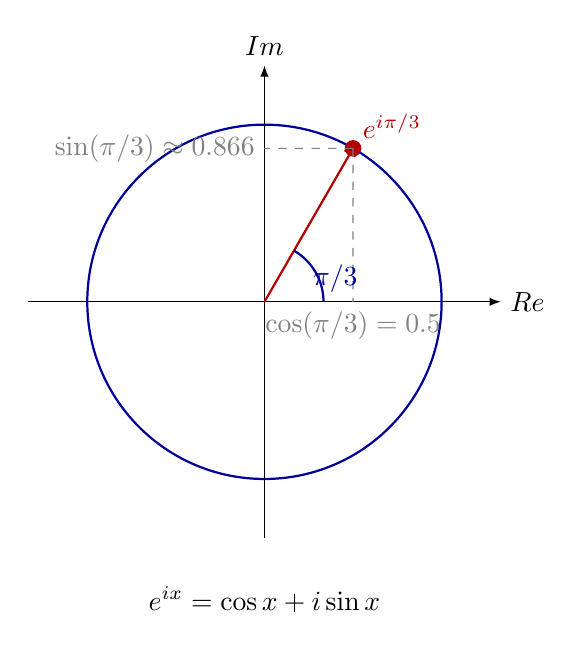
\begin{tikzpicture}[scale=1.5]
  % Unit circle
  \draw[blue!60!black, thick] (0,0) circle (1.5cm);
  
  % Axes
  \draw[->, >=latex] (-2,0) -- (2,0) node[right] {$\operatorname{Re}$};
  \draw[->, >=latex] (0,-2) -- (0,2) node[above] {$\operatorname{Im}$};
  
  % Point e^(ix) at angle pi/3
  \coordinate (P) at ({1.5*cos(60)},{1.5*sin(60)});
  \draw[red!70!black, thick, ->] (0,0) -- (P);
  \fill[red!70!black] (P) circle (2pt);
  
  % Projections
  \draw[dashed, gray] (P) -- ({1.5*cos(60)},0);
  \draw[dashed, gray] (P) -- (0,{1.5*sin(60)});
  
  % Labels
  \node[red!70!black, above right] at (P) {$e^{i\pi/3}$};
  \node[below, gray] at ({1.5*cos(60)},0) {$\cos(\pi/3) = 0.5$};
  \node[left, gray] at (0,{1.5*sin(60)}) {$\sin(\pi/3) \approx 0.866$};
  
  % Angle arc
  \draw[blue!60!black, thick] (0.5,0) arc (0:60:0.5);
  \node[blue!60!black] at (0.6,0.2) {$\pi/3$};
  
  % Formula
  \node[below=0.5cm] at (0,-2) {$e^{ix} = \cos x + i\sin x$};
\end{tikzpicture}
